%% Requires compilation with XeLaTeX or LuaLaTeX
%% based on UC Berkeley Beamer theme https://www.overleaf.com/latex/templates/uc-berkeley-beamer-theme/bywswngntrws
\documentclass[10pt,xcolor={table,dvipsnames},t]{beamer}

\usetheme{UCBerkeley}
\setbeamertemplate{footline}[frame number] 
\RequirePackage[style=numeric]{biblatex}
\addbibresource{refs.bib}
\RequirePackage{csquotes}
\RequirePackage{amsmath}
\RequirePackage{physics}
\RequirePackage{graphicx}
\RequirePackage[font=small]{caption, subcaption}
\RequirePackage{wrapfig}
\RequirePackage{siunitx}
\RequirePackage{sidecap}
\RequirePackage{caption}
\RequirePackage{booktabs}
\RequirePackage{xcolor}
\definecolor{officeblue}{RGB}{53, 136, 195}
\captionsetup[figure]{font = scriptsize, labelfont = scriptsize} % https://tex.stackexchange.com/questions/52132/beamer-change-size-of-figure-caption
\setkeys{Gin}{width=1\linewidth}


\title[Autosailboat]{Autonomous control of a sailboat}
\author{Neelay Junnarkar, Andrew Fearing, Hamza Khawaja}
% \institute{Your Faculty/Department}
\date{\today}

\begin{document}

\begin{frame}
  \titlepage
\end{frame}

\begin{frame}{Outline}
 \tableofcontents
\end{frame}
\section{Introduction}
% \begin{frame}{Team}
% 
% Neelay Junnarkar
% 
% \hfill\\
% Andrew Fearing
% 
% \hfill\\
% Hamza Khawaja
% \end{frame}

\subsection{Background}
\begin{frame}{Motivation}
\begin{columns}
\column{0.5\linewidth}
    \begin{figure}
        \centering
        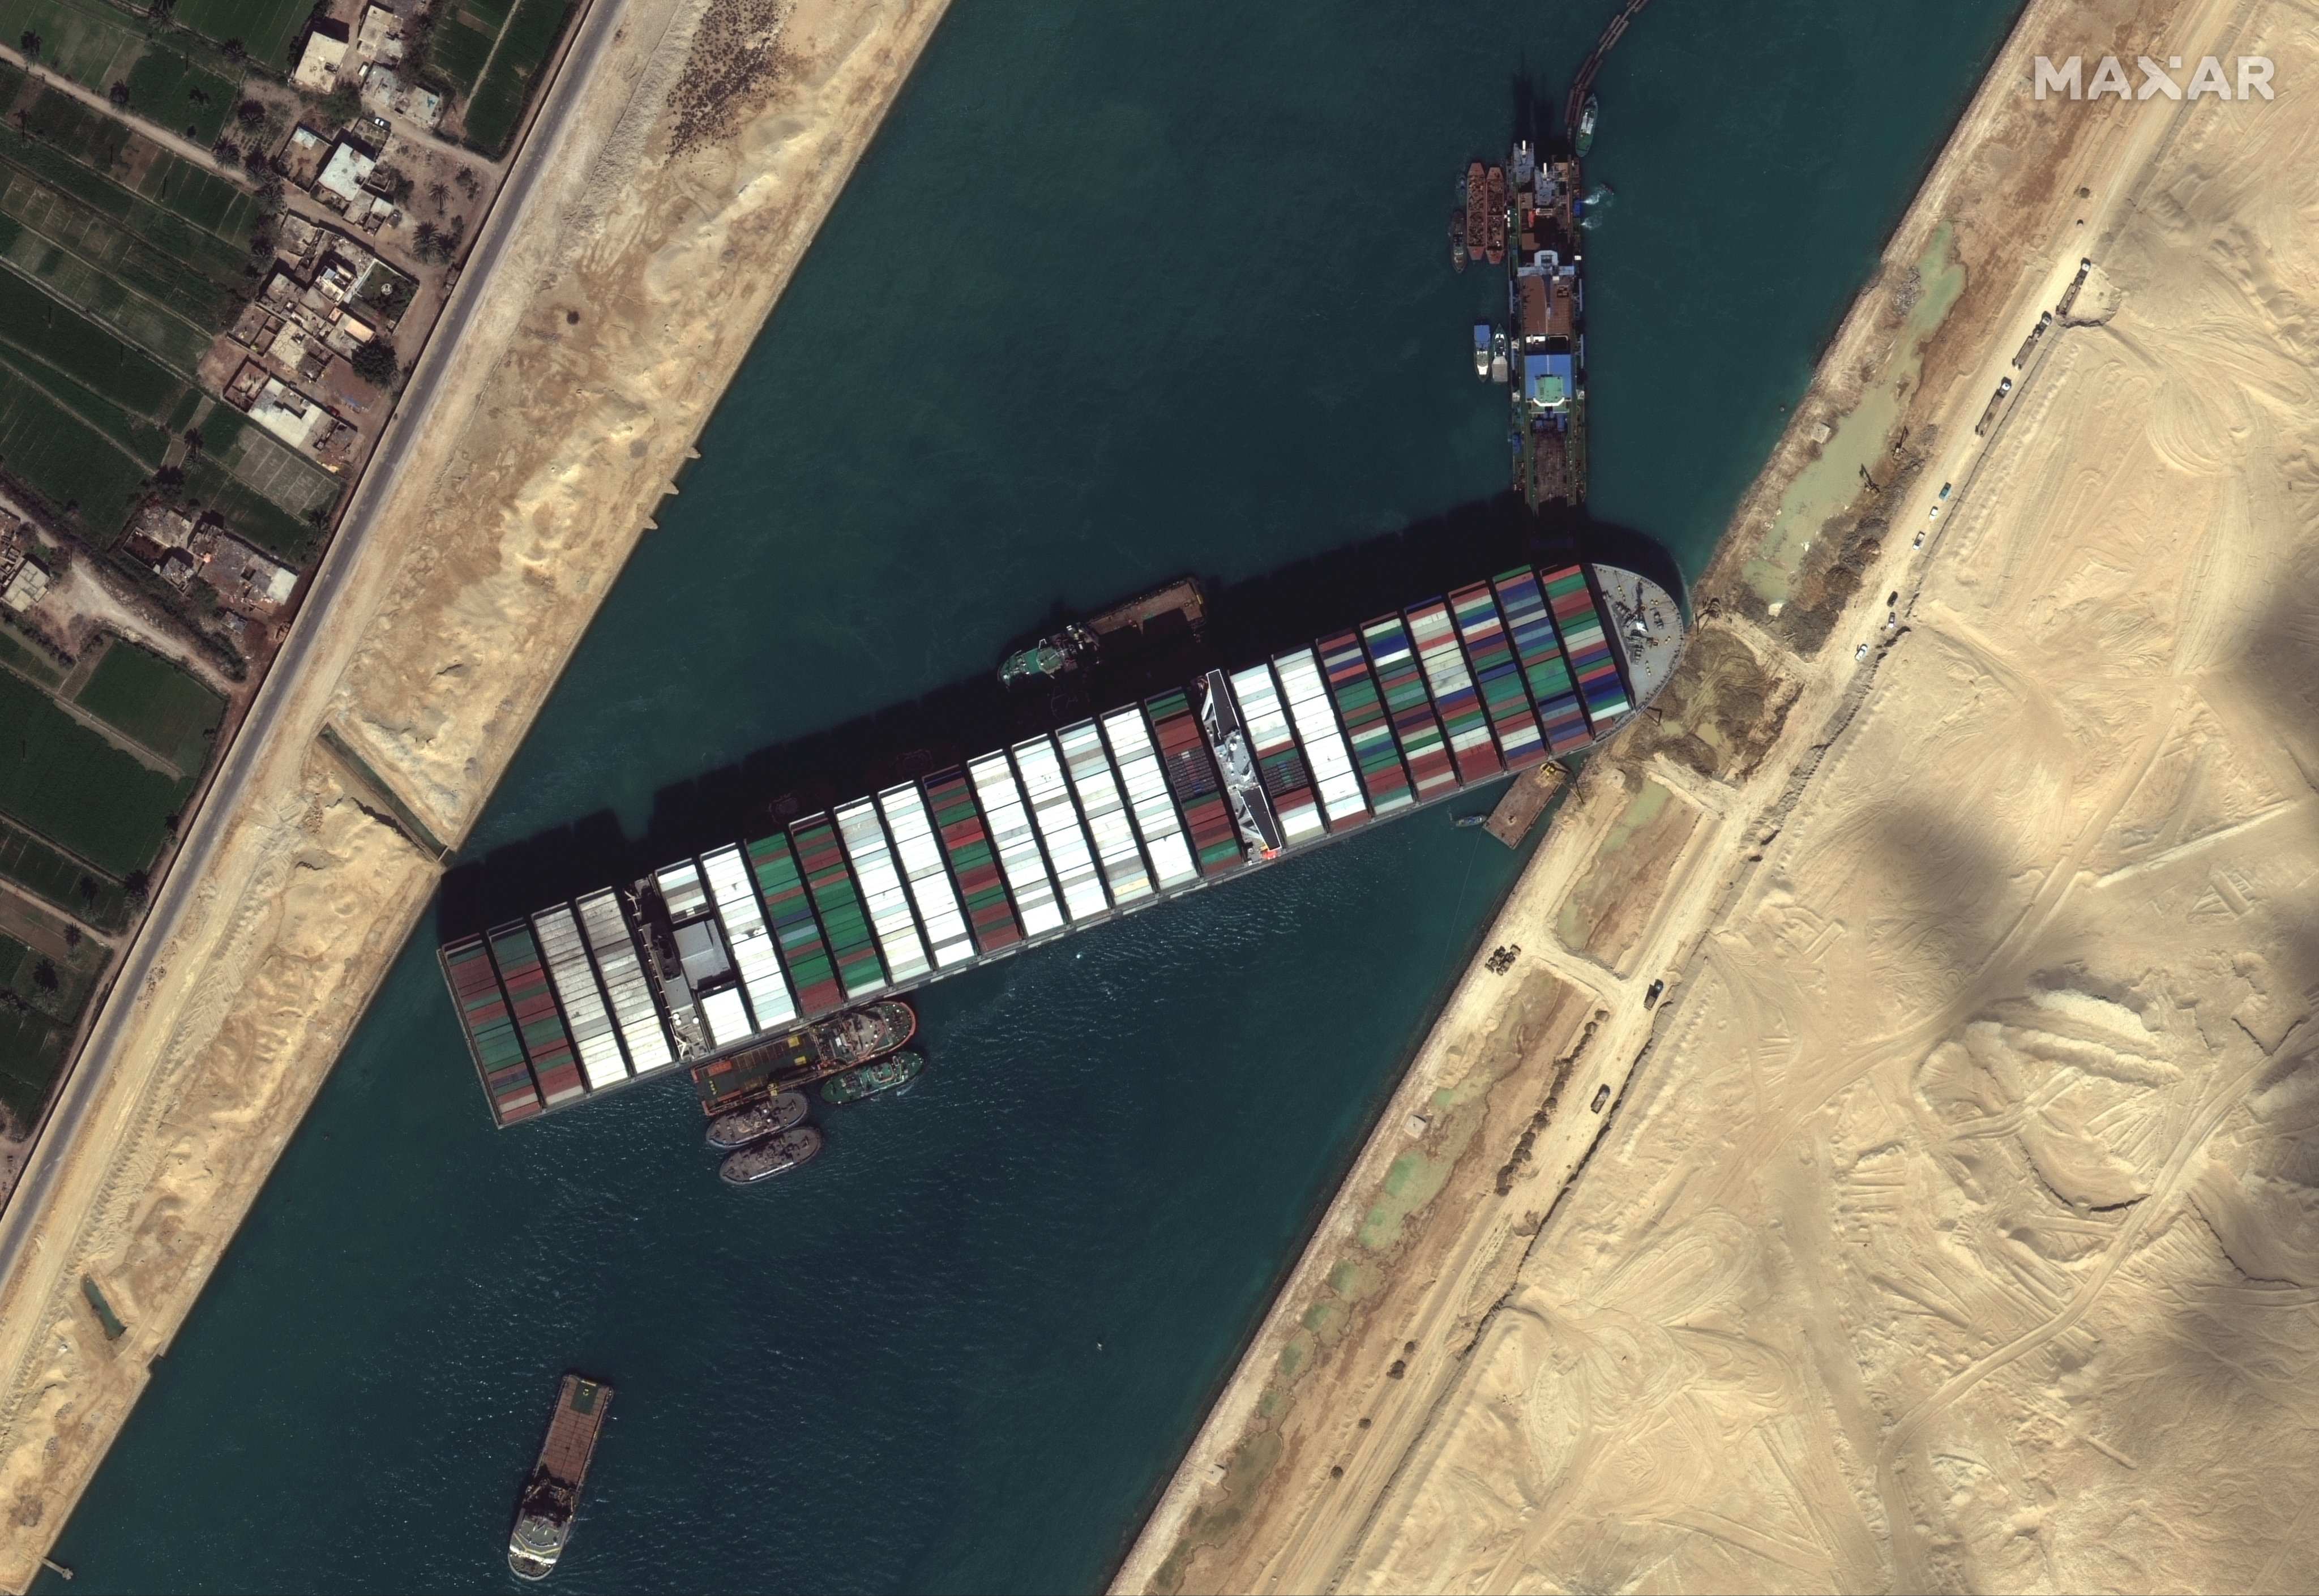
\includegraphics{documents/figures/Suez_Canal_blocked_by_Ever_Given_March_27_2021.jpg}
        \caption{Boat stuck}
        \label{fig:boat_stuck}
    \end{figure}  
\column{0.5\linewidth}
    \textbf{Why Sailboats?}
    
    \hfill\\
    Sailboats are useful for low-power long-term deployments. Also, present a gap in current literature,
    especially in controller design.
    \\
\hfill\\
    \textbf{Control of sailboats}
    
    \hfill\\
    Controlling boats autonomously presents an interesting challenge due to the large effect of environmental disturbances such as wind, water currents, and waves. 
    
    

    
\end{columns}
\end{frame}

\begin{frame}{Goal}

Develop planning and control scheme which can take into account environmental disturbances and obstacles such as channels.

\end{frame}
  

\begin{frame}{Sailing}
\begin{columns}
\column{0.5\linewidth}

\begin{figure}
    \centering
    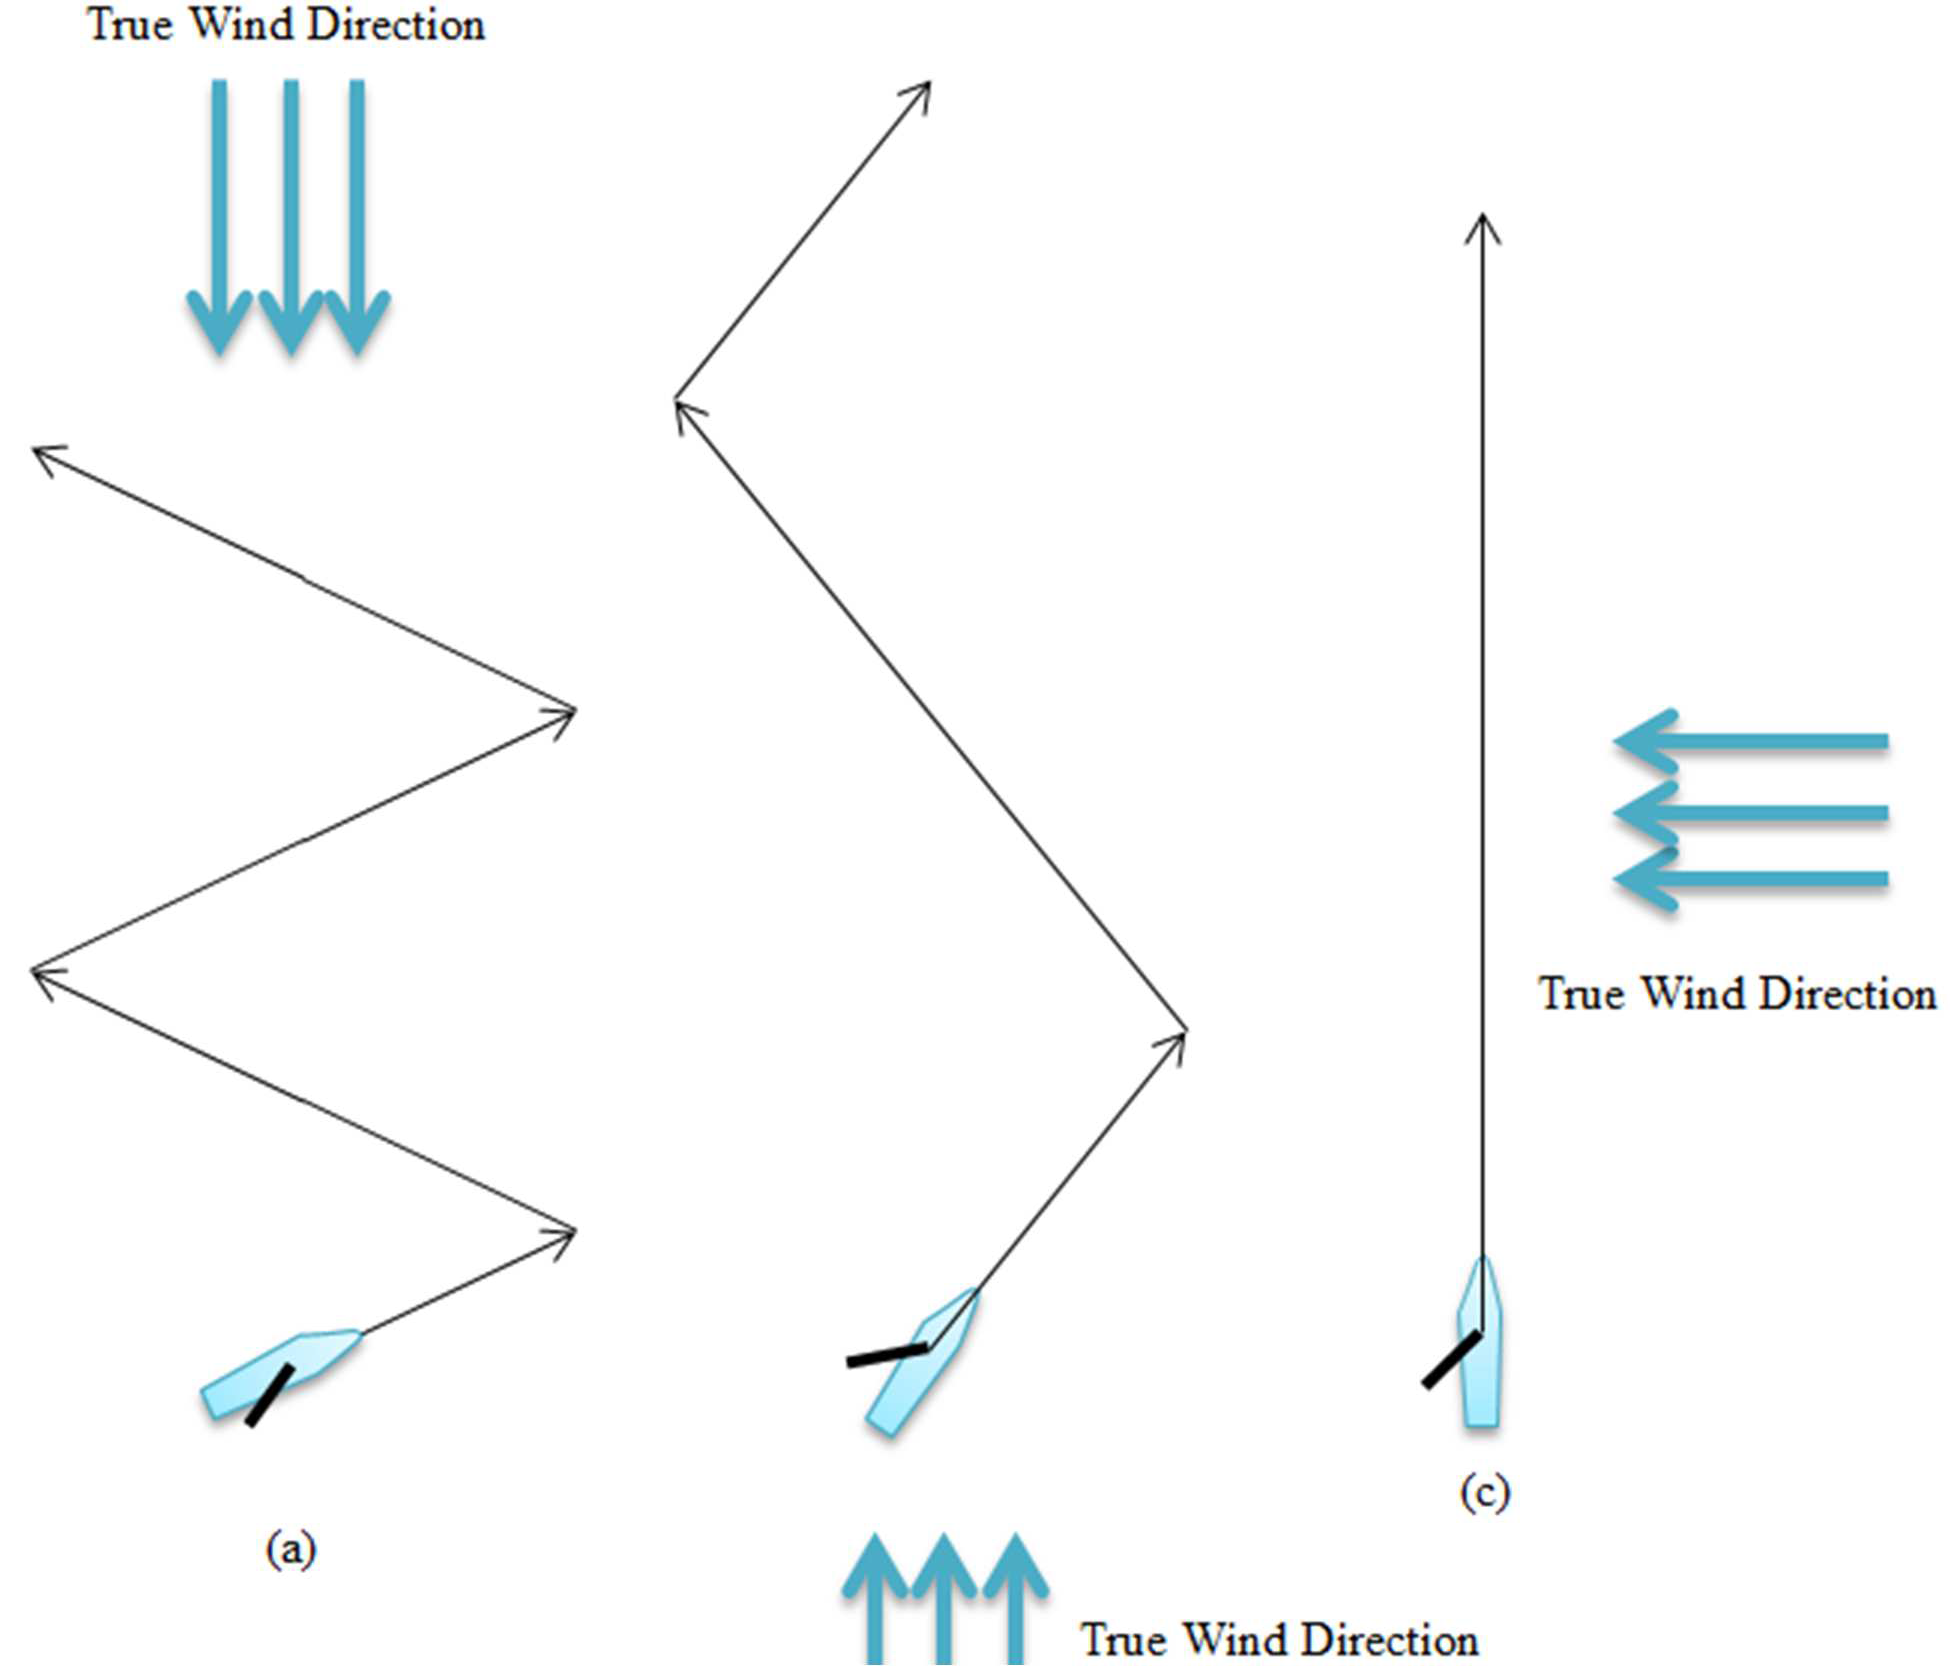
\includegraphics[width=\linewidth]{documents/figures/alves_modes.png}
    \caption{Modes of sailing \cite{Alves2010}}
    \label{fig:alves_modes}
\end{figure}
\column{0.5\linewidth}
\begin{figure}
    \centering
    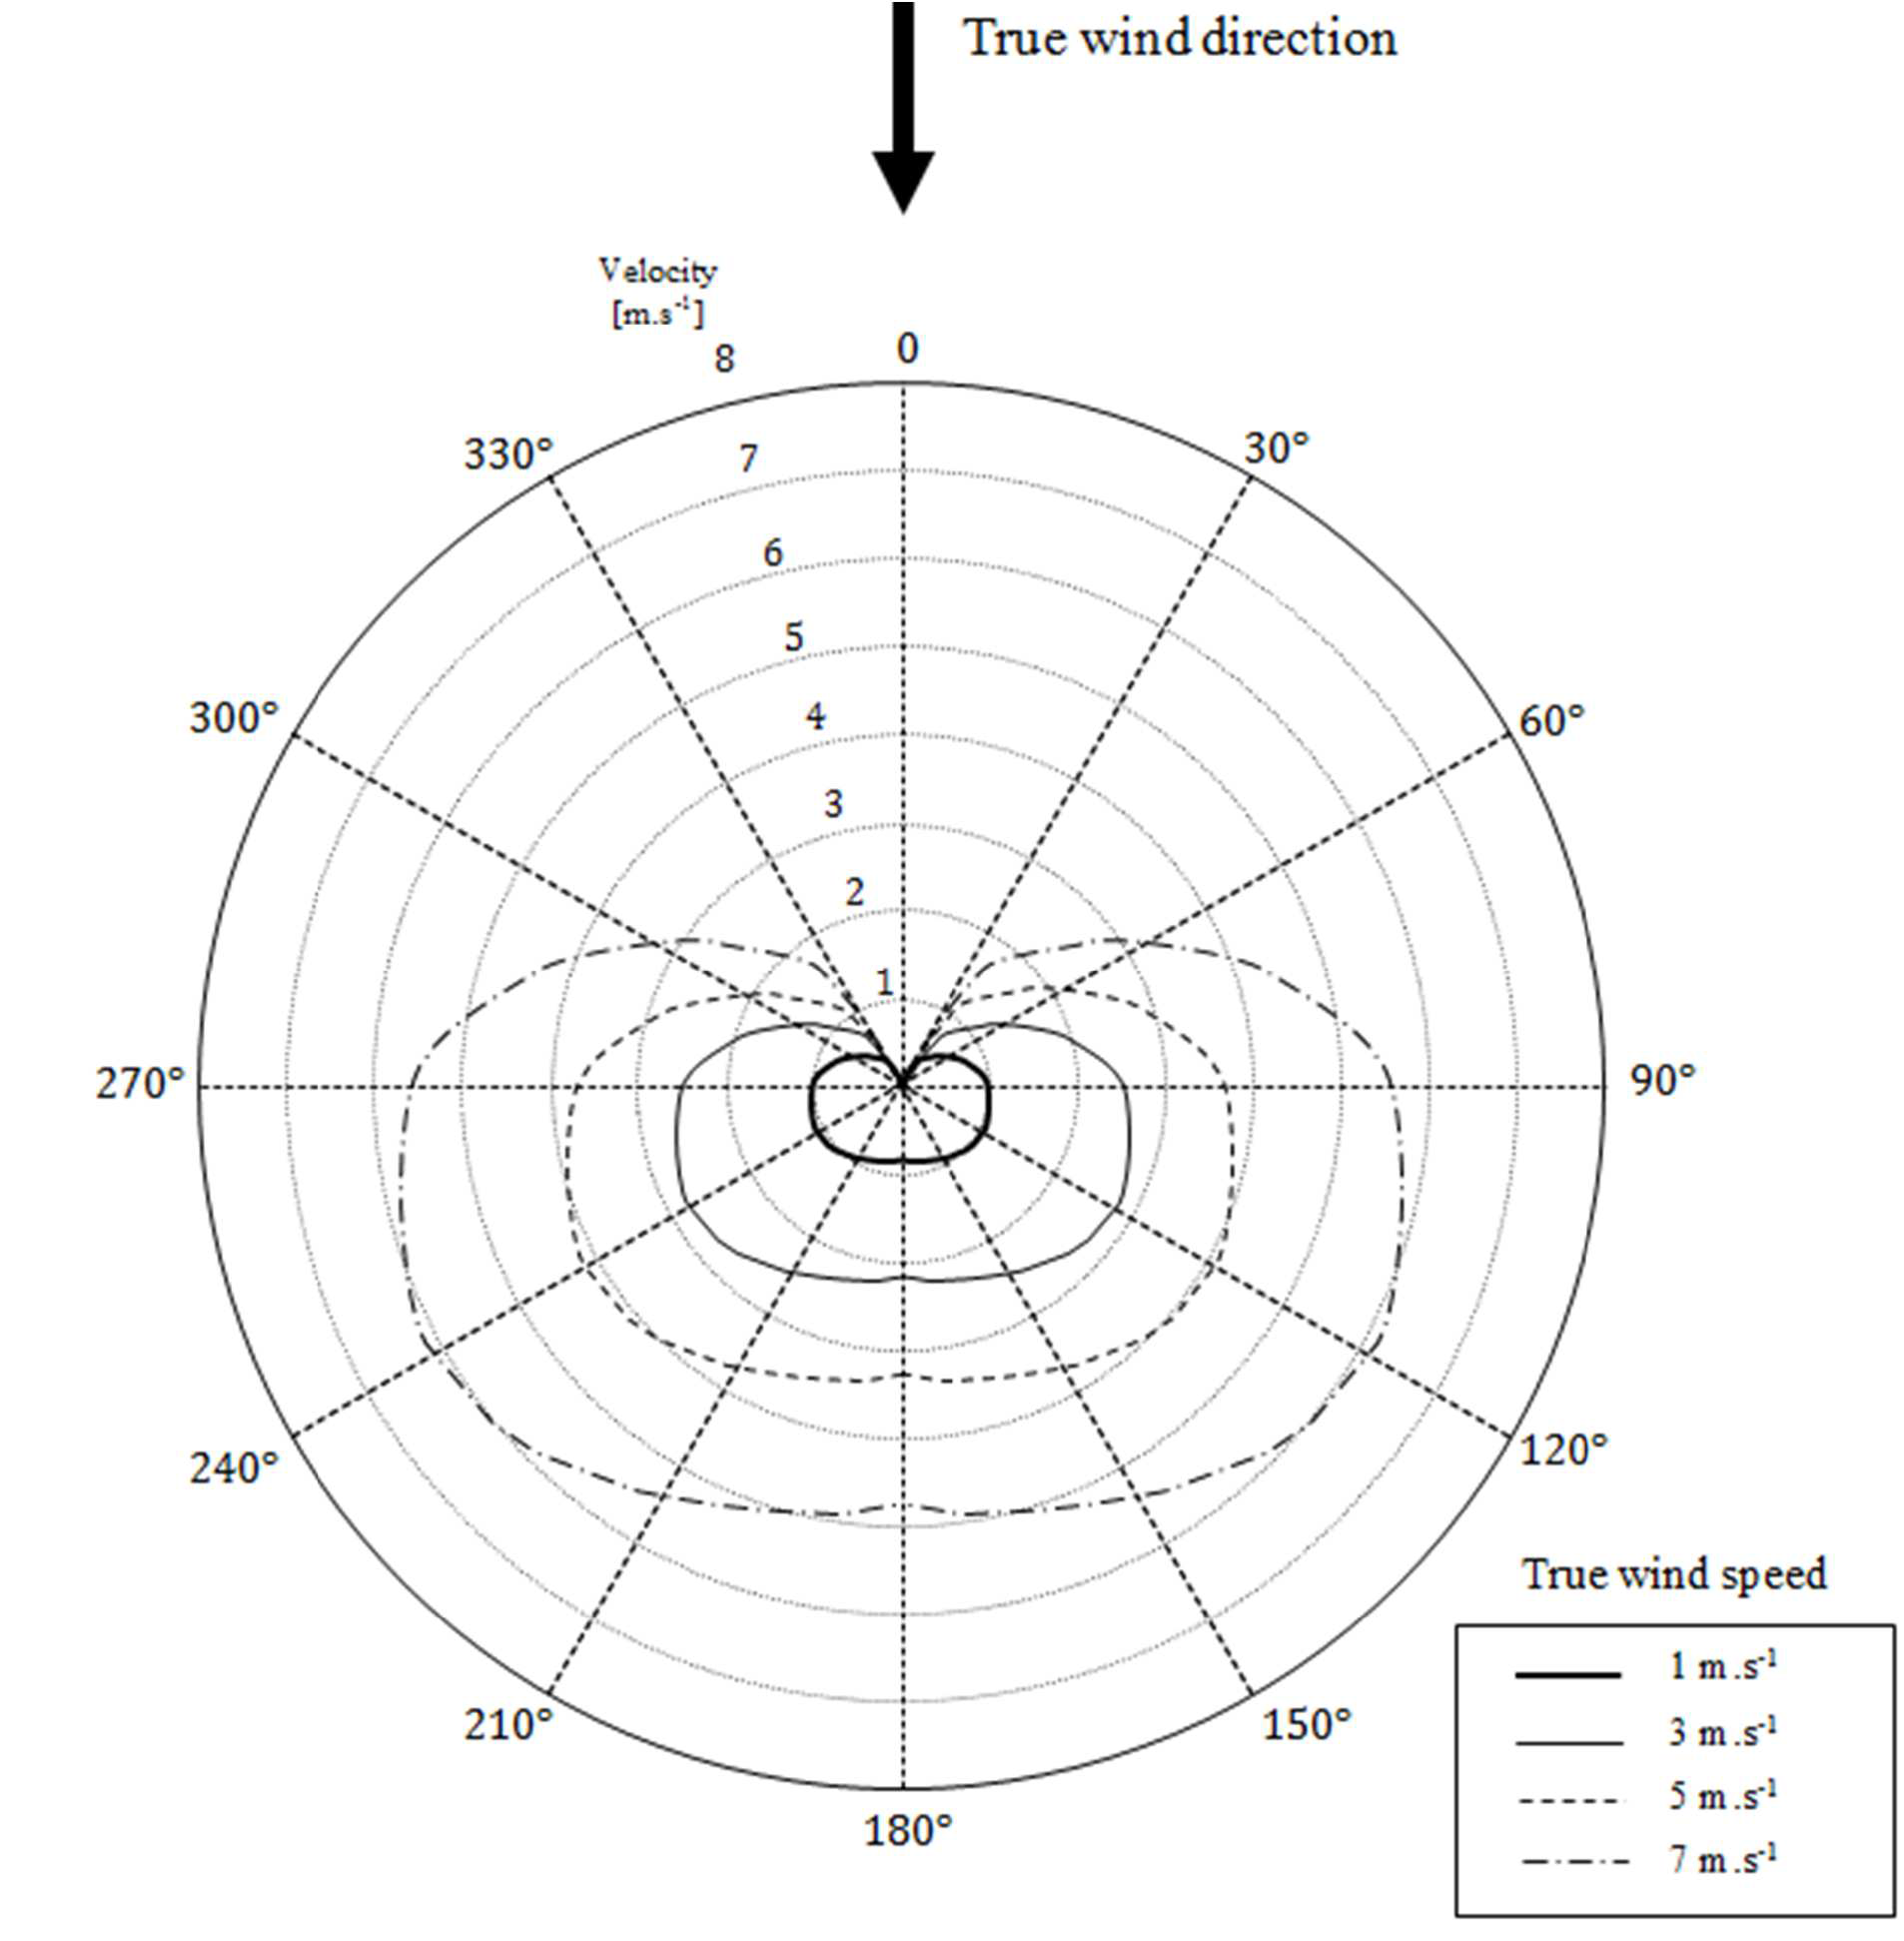
\includegraphics[width=\linewidth]{documents/figures/alves_vpp.png}
    \caption{Velocity polar diagram \cite{Alves2010}}
    \label{fig:alves_velocity}
\end{figure}
\end{columns}
\centerline{Sailboats trajectories depend on wind direction}
\end{frame}

\subsection{Sailboat model}

\begin{frame}{Sailboat Components}
\begin{columns}
\column{0.5\linewidth}
    \begin{figure}
        \centering
        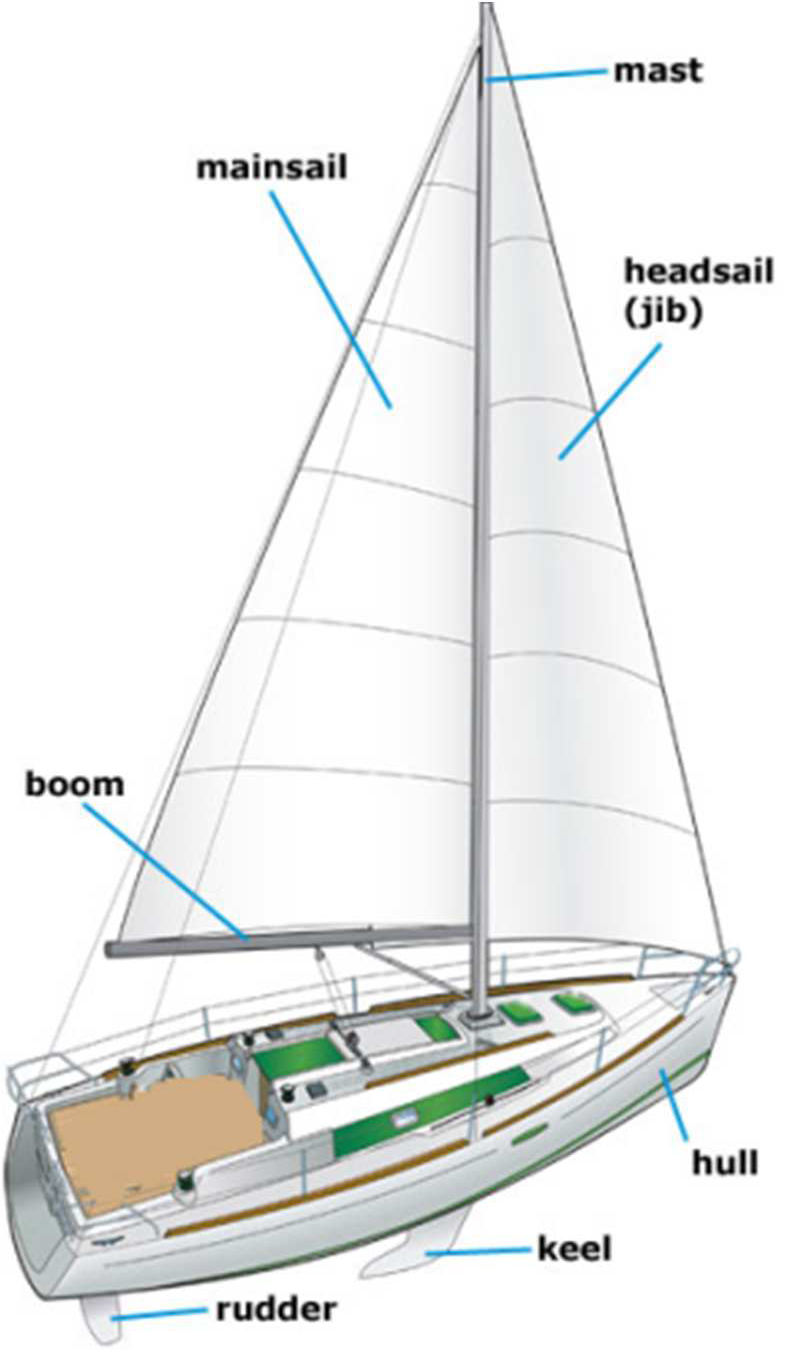
\includegraphics[height = 0.6\textheight, keepaspectratio]{documents/figures/alves_sailboat.png}
        \caption{Sailboat main components~\cite{Alves2010}.}
        \label{fig:my_label}
    \end{figure}
\column{0.5\linewidth}
\begin{itemize}
    \item Note that headsail and mainsail are connected in our model for simplicity
    \item Two control surfaces: sail and rudder \(\implies\) two actuators
\end{itemize}
\end{columns}

\end{frame}

\begin{frame}{6-DoF Model Axes and State Space}
\begin{columns}
\column{0.4\linewidth}
\begin{figure}
    \centering
    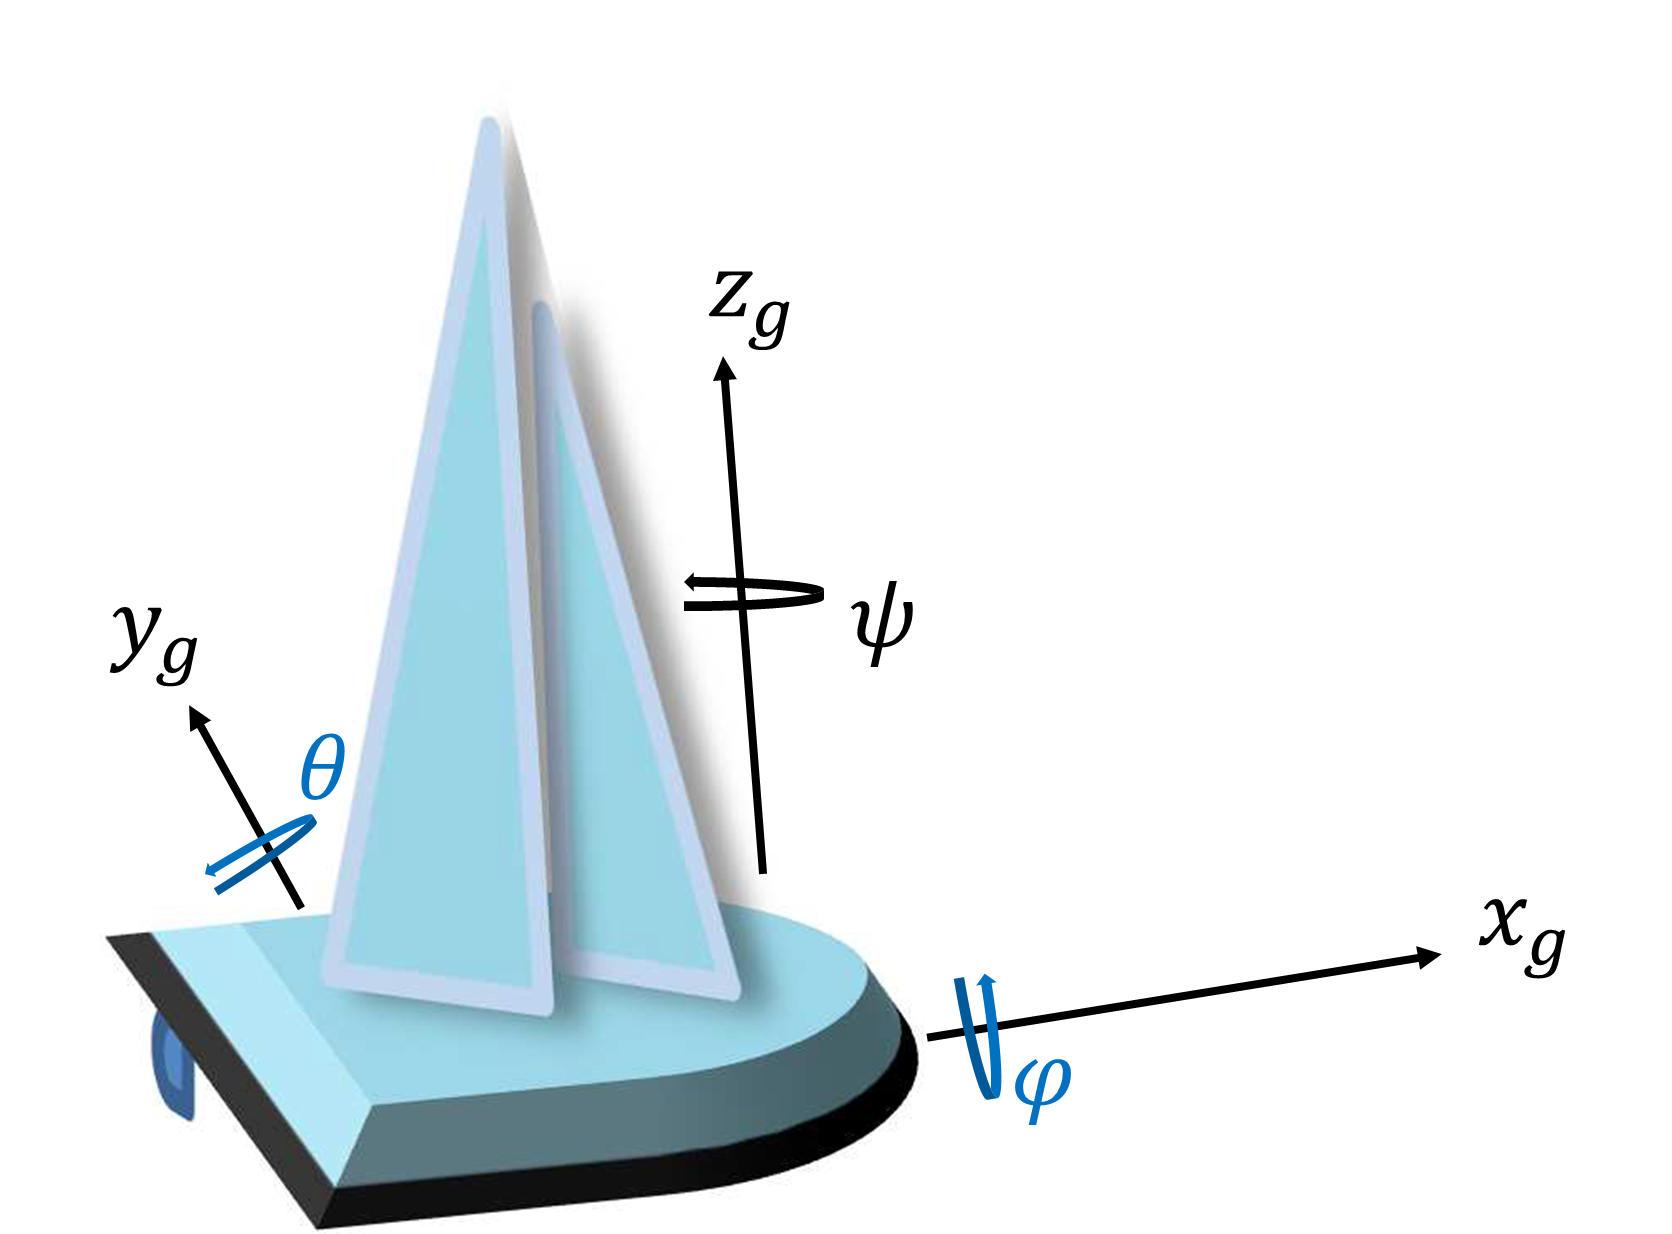
\includegraphics[width = \linewidth, height = \textheight, keepaspectratio]{documents/figures/alves_boat_with_buehler_axes.png}
    \caption{Sailboat axes~\cite{Alves2010}}
    \label{fig:sailboat_components}
\end{figure}
\begin{tabular}{ll}
\textcolor{black}{\(\blacksquare\)}& Global frame \\
     \textcolor{officeblue}{\(\blacksquare\)}& Boat frame 
\end{tabular}
\column{0.6\linewidth}
\begin{table}
    
    \centering
    \begin{tabular}{ccc}
    name & position & velocity \\
     &\(x_g\) & \(v_x\) \\
     &\(y_g\) & \(v_y\) \\
     &\(z_g\) & \(z_x\) \\
     heading&\(\psi\) & \(p\) \\
     \textcolor{officeblue}{roll} & \textcolor{officeblue}{\(\theta\)} & \textcolor{officeblue}{\(q\)} \\
     \textcolor{officeblue}{pitch}&\textcolor{officeblue}{\(\varphi\)} & \textcolor{officeblue}{\(r\)} \\
     \textcolor{officeblue}{rudder angle} & \textcolor{officeblue}{\(\rho\)} & \\
     \textcolor{officeblue}{sail angle}   & \textcolor{officeblue}{\(\gamma\)} & 
    \end{tabular}
    \caption{The 14 sailboat state variables~\cite{Buehler2018}.}
    \label{tab:state_vars}
\end{table}


\end{columns}

    
\end{frame}

\begin{frame}{Dynamics Model}

Position:
\begin{equation}
    \dv{t} \mqty(x_g \\ y_g \\ z_g) = \mqty(v_x \cos(\psi) - v_y \sin(\psi) \\ v_x \sin(\psi) + v_y \cos(\psi) \\ v_z)
\end{equation}

Angles:
\begin{equation}
    \dv{t} \mqty(\varphi \\ \theta \\ \psi) \approx \mqty(p \\ \cos(\varphi) q - \sin(\varphi) r \\ \cos(\varphi) r + \sin(\varphi) q)
\end{equation}

Velocities:
\begin{equation}
    m\dv{t}\mathbf{v} = \mathbf{F}
\end{equation}

Angular Velocities:
\begin{equation}
    \dv{t}(\Theta\Omega) = \mathbf{T} = \sum_i r_i \times \mathbf{F}_i
\end{equation}

Forces and torques are derived from physical interactions of environment, sailboat, sail, and rudder.
\end{frame}

\begin{frame}{Control Surfaces}

\begin{columns}
\column{0.4\linewidth}
\begin{figure}
    \centering
    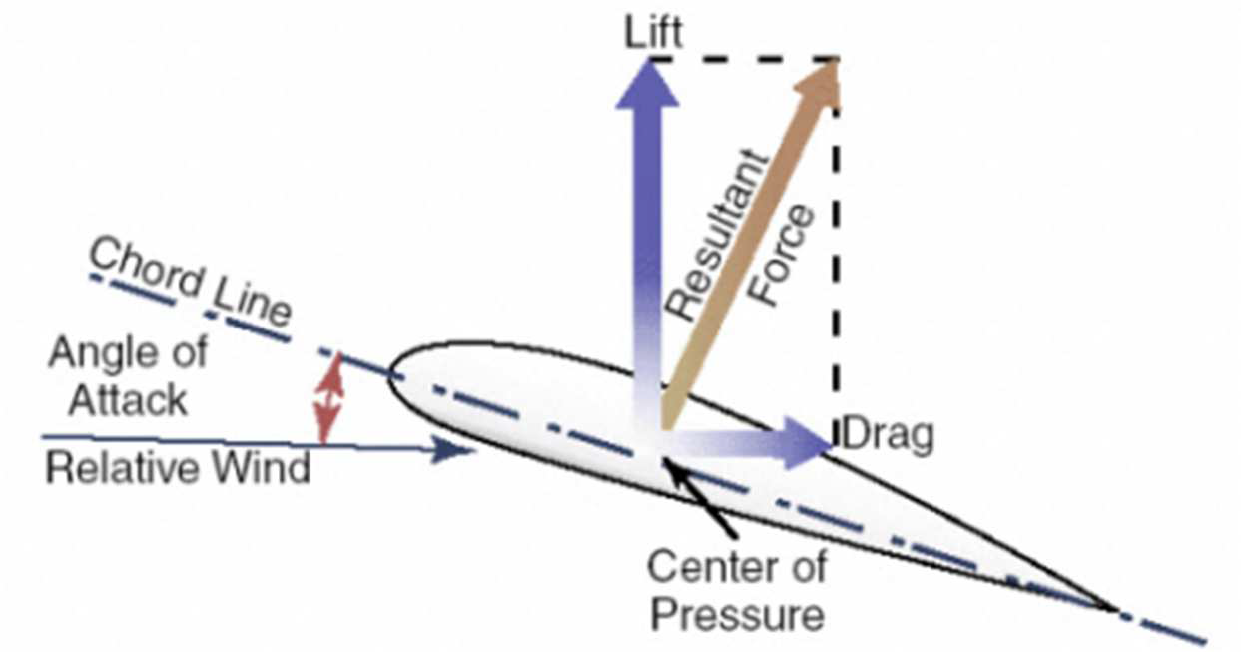
\includegraphics[width = \linewidth]{documents/figures/alves_wing.png}
    \caption{Drag and lift forces on a foil~\cite{Alves2010}.}
    \label{fig:alves_foil}
\end{figure}



\column{0.6\linewidth}

Because the boat is moving, foils have \enquote{apparent velocity} in fluid\\\textbf{}
\begin{equation}
    \mathbf{V}_{af} = \mathbf{V}_f - \mathbf{V}
\end{equation}
\(\mathbf{V}_{af}\) is the apparent velocity of the foil relative to the fluid\\
\(\mathbf{V}_{f}\) is the velocity of the fluid\\
\(\mathbf{V}\) is the velocity of the sailboat
\end{columns}
\hfill{} \\
\begin{equation}
    \mathbf{F}_{\mathrm{flow}} = \frac{1}{2} \rho v_{rel}^2 A \mqty(\sin(\beta) c_L - \cos(\beta) c_D \\ \sin(\beta) c_D + \cos(\beta) c_L\\ 0)
\end{equation}
where \(C_L\) and \(C_D\) are lift and drag coefficients, respectively; \(\beta\) is the apparent flow angle; \(A\) is the foil area; and \(\rho\) is the fluid mass density.
\end{frame}

\begin{frame}{Control Surfaces, continued}
    \begin{columns}
    \column{0.4\linewidth}
    \begin{figure}
        \centering
        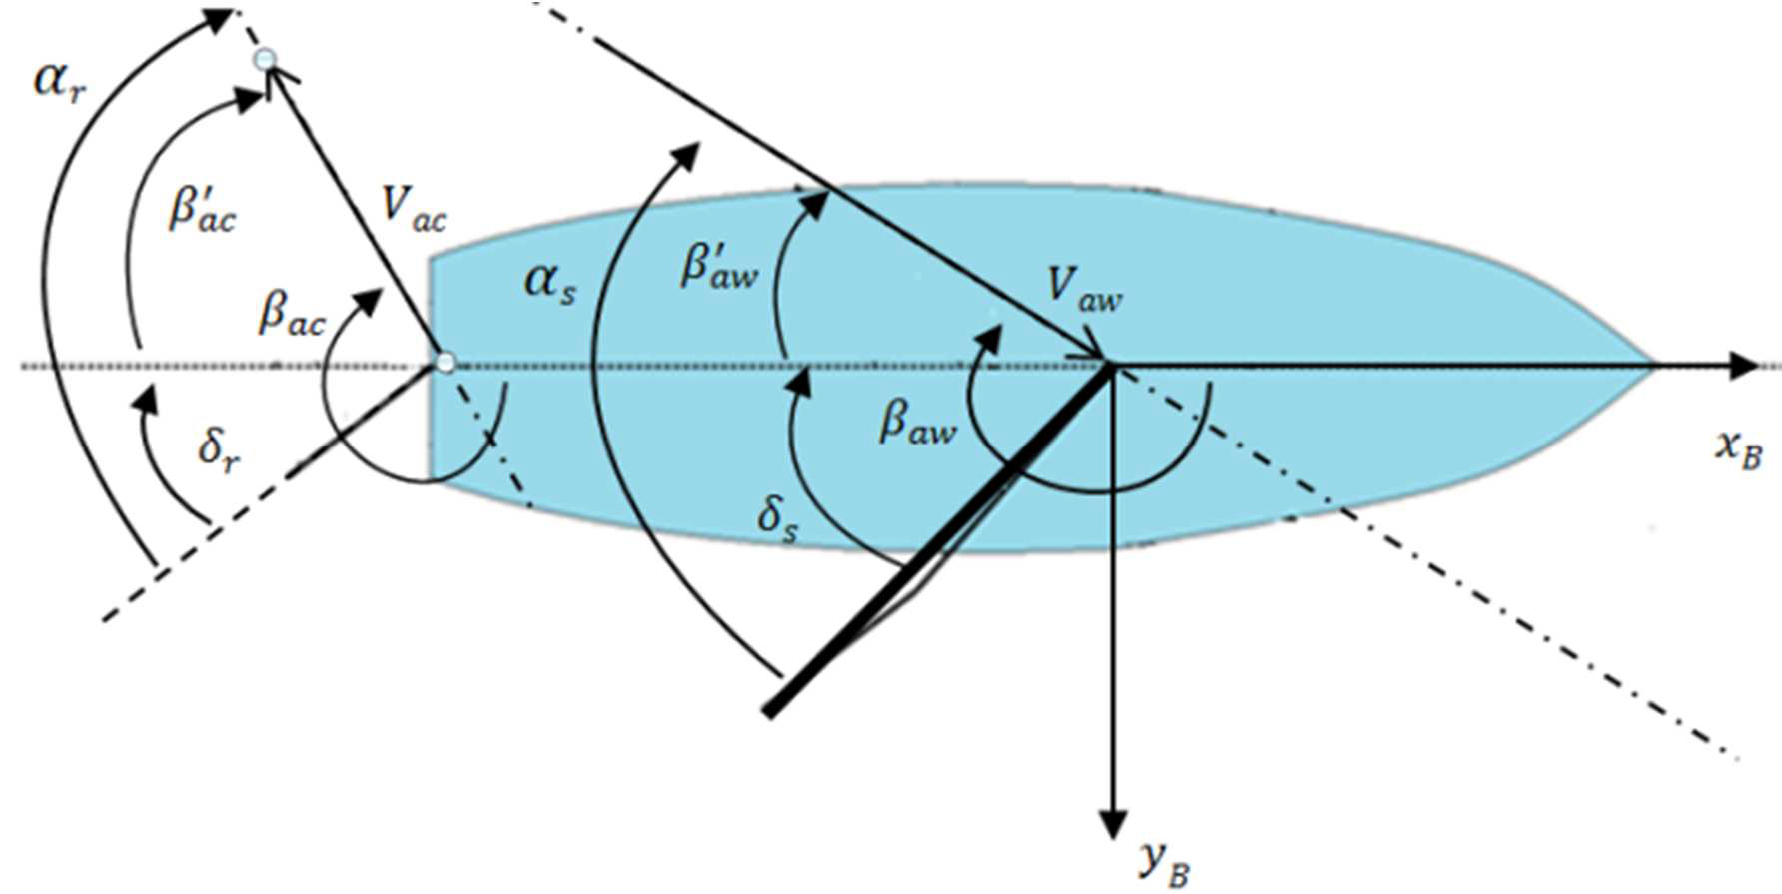
\includegraphics{documents/figures/alves_sailboat_angles.png}
        \caption{Control surface angles~\cite{Alves2010}.}
        \label{fig:my_label}
    \end{figure}
    \column{0.6\linewidth}
    \centerline{Bottom line}
    \begin{itemize}
        \item Set set angle to maximize wind force -- use geometry
        \item Rudder induces moment about \(z)\) - axis -- relies on keel
    \end{itemize}

    \end{columns}
    \centerline{\(\therefore\) Only need to control rudder}
\end{frame}

\subsection{Simulator}
\begin{frame}{Evaluating Simulators}
    
    
    Simulators for sailboat models are significantly underdeveloped.
    
    \begin{columns}
    \column{0.5\linewidth}
        \centerline{\texttt{USVSim} \cite{Paravisi2019}}
        \begin{itemize}
            \item Ubuntu 16.04 + Kinetic ROS + Gazebo
            \item 6 DoF boat dynamics model.
            \item Waves, buoyancy, water currents, wind currents, thruster underwater, thruster above water, foil.
            \item Too complicated to work with, hard to extend.
        \end{itemize}
    \column{0.5\linewidth}
        \centerline{\texttt{stda-sailboat-sim} \cite{Buehler2018}}
        \begin{itemize}
            \item Python + Numpy + Matplotlib
            \item 6 DoF boat dynamics model.
            \item Waves, buoyancy, wind, sail, keel, rudder forces.
            \item Good enough .
        \end{itemize}

    \end{columns}
    
\end{frame}



% \begin{frame}{Refactoring Simulator}
% 
%     \texttt{stda-sailboat-sim} simulator appears to have been written just enough to satisfy the needs of the authors paper.
%     
%     \hfill\\
%     We rewrote it significantly to modularize the code and allow easy and structured definition
%     of controllers and path planners.
% 
% \end{frame}

% \begin{frame}{Simulation Results}
% \begin{table}[h]
%     \centering
%     \begin{tabular}{lcc}
%     x-y trajectory & 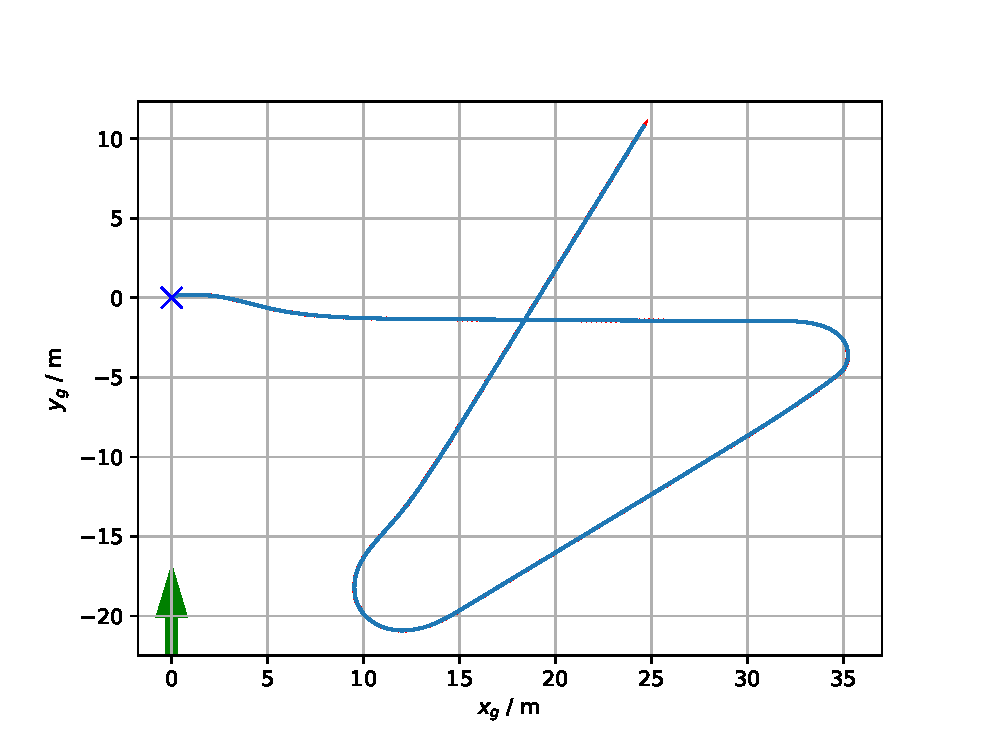
\includegraphics[width = 0.35\linewidth]{documents/figures/trajectories.eps} &
%     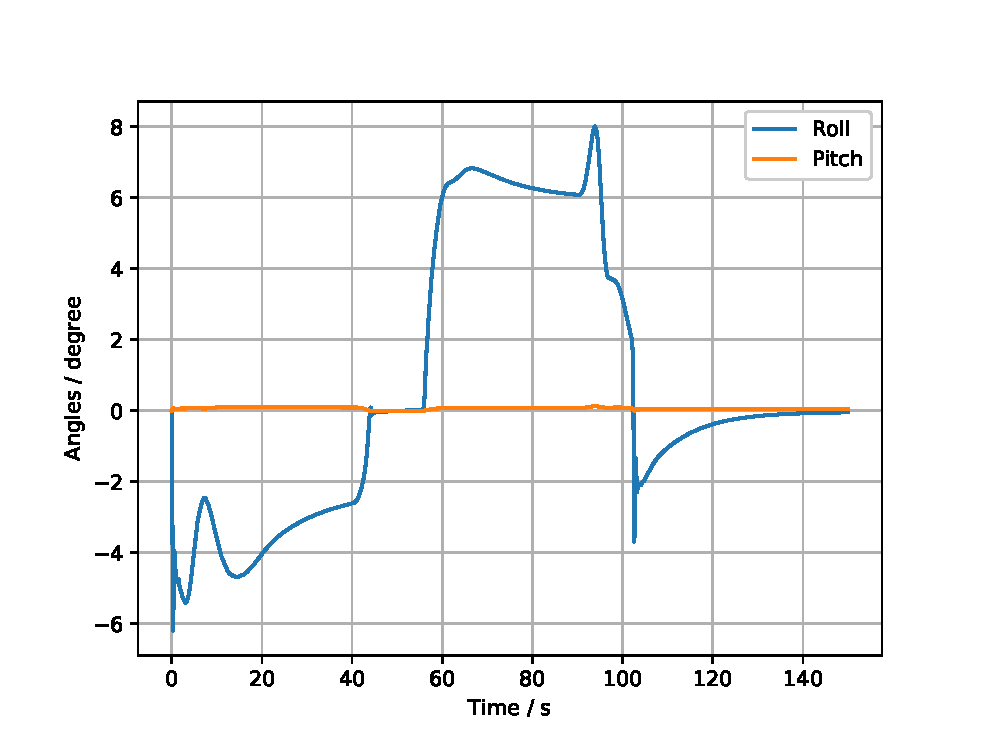
\includegraphics[width = 0.35\linewidth]{documents/figures/angles.eps} \\
%     heading angle & 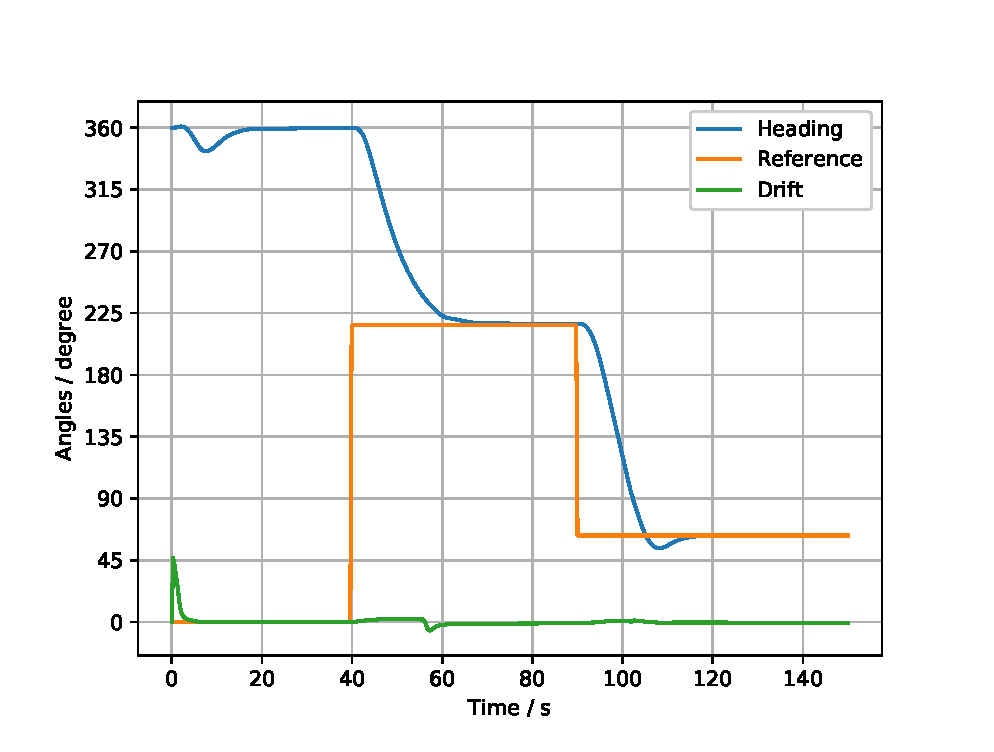
\includegraphics[width = 0.35\linewidth]{documents/figures/heading.eps} & 
%     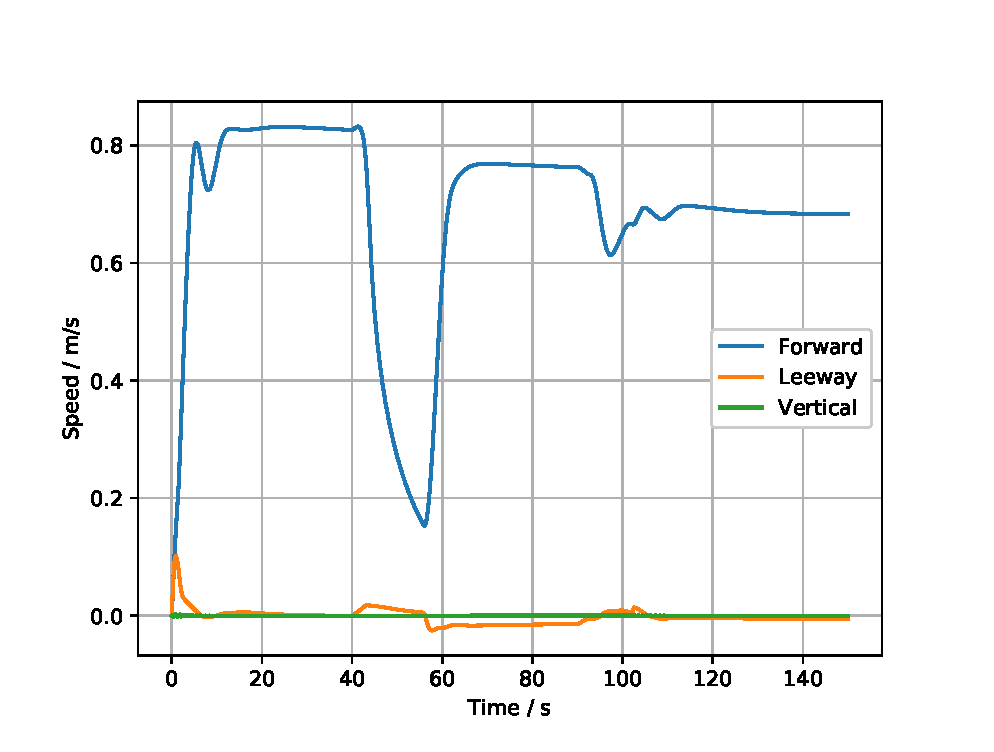
\includegraphics[width = 0.35\linewidth]{documents/figures/speeds.eps}
%     \end{tabular}
%     \caption{Simulator results with example reference headings}
%     \label{tab:plots  }
% \end{table}
% \end{frame}


\section{Control Design}

\begin{frame}{High-level Control Design}

\begin{figure}
    \centering
    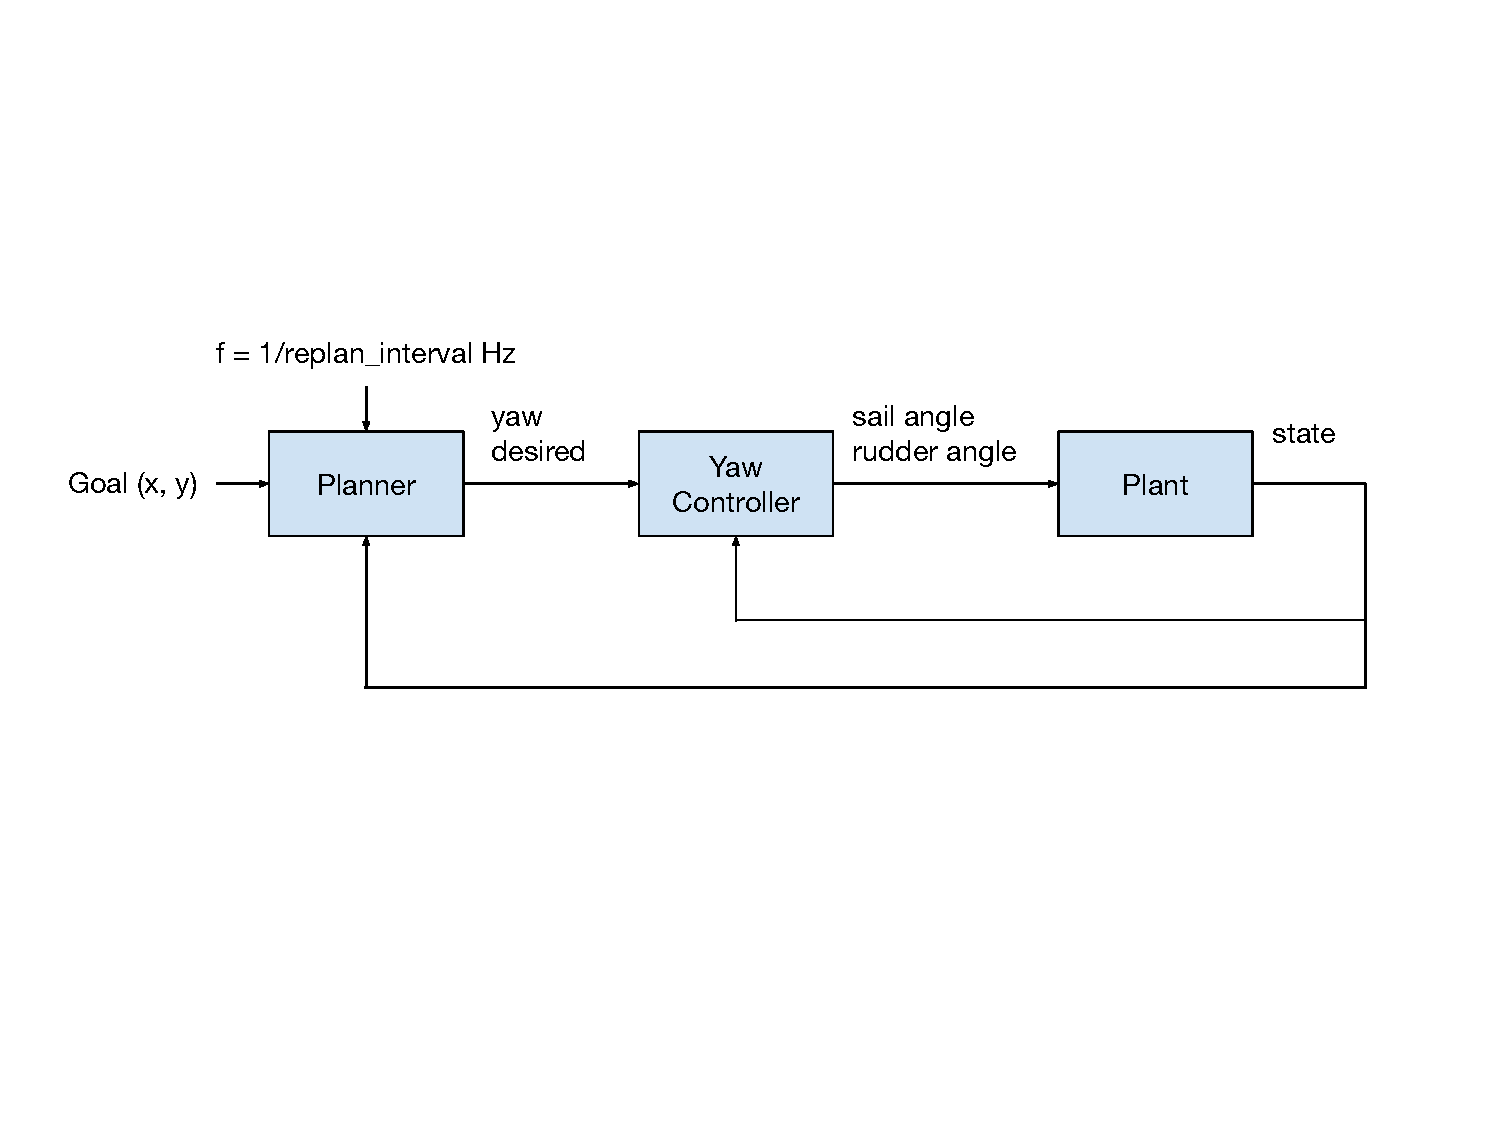
\includegraphics[width=\linewidth,trim={1cm 7cm 2cm 5cm},clip]{documents/final_pres_figs/controller_block_diagram.pdf}
    \caption{Block diagram of planner and controller}
    \label{fig:controller_block_diagram}
\end{figure}
    
A planner generates a reference heading (yaw) for the boat to reach a given \(x, y\) coordinate goal
and boat state.
The planner is run at a low rate since planning, and also the boat itself, is slow.

\hfill\\
The yaw controller generates sail angles and rudder angles to be used as inputs to the boat to
track the reference heading.

\end{frame}

\begin{frame}{Yaw Controller}

    Yaw controller tracks a reference yaw by setting sail and rudder angles.

    \hfill\\
    Implemented as per the same paper which developed the simulator and 
    boat dynamics model we are using\cite{Buehler2018}.
    
    \hfill\\
    This controller leverages the fact that there is an optimal angle for the sail based on wind direction to  the rudder and sail angle control.
    
    \hfill\\
    Note that the inputs called here as `rudder angle' and `sail angle' are actually
    inputs to a first order model that simulates delays in changing the rudder and sail angles.
    
\end{frame}

\begin{frame}{Yaw Controller}

    Apparent wind is the wind relative to the boat (accounting for boat velocity).
    
    \hfill\\
    With \(\theta_{aw}\) being the angle of the apparent wind, sail angle is optimally set based on current boat yaw as 
    \begin{equation}
        \theta_{\text{sail}} = \frac{\sin(\theta_{aw})}{\cos(\theta_{aw}) + 0.4\cos^2(\theta_{aw})}
    \end{equation}
    This is clipped based on sailboat limit.

    \hfill\\
    The rudder controller is implemented as a PID controller derived from a Jacobian linearization of a simplified dynamics model from input rudder to output yaw.
    
    \hfill\\
    Gains are determined through LQR.
    
\end{frame}

\begin{frame}{Planner}
    
    The planner takes in a high level \(x, y\) goal and plans a yaw trajectory for the boat 
    to reach the goal.
    
    \hfill\\
    We design the planner as repeatedly solving constrained nonlinear optimization problems with receding horizons. Due to model complexity, the planner runs slowly and so we define a 
    replanning interval on the order of 10s of seconds.
    
    \hfill\\
    Objective: the standard LQR-like quadratic objective with \(Q\) and \(R\) tunable cost matrices.
    
    \hfill\\
    Constraints: planned path must satisfy simplified boat dynamics and avoid obstacles.
    
    \hfill\\
    The optimization problems are solved with Casadi and the IPOPT solver.
    
\end{frame}

\begin{frame}{Planner: Boat Model}

    A simplified boat dynamics model is used in the planner to speed up planning.
    Also, some information used by the boat dynamics model are not well known 
    ahead of time.
    
    \hfill\\
    We make a simplified 3 state boat dynamics model with states \(x, y, \psi\) where 
    \(x, y\) are position and \(\psi\) is heading, and a non-physical input \(u\) 
    such that 
    
    \begin{equation}
        \mqty[\dot{x} \\ \dot{y} \\ \dot{\psi}]
         = \mqty[v_x \cos(\psi) - v_y \cos(\psi) \\ 
         v_x \sin(\psi) + v_y\cos(\psi) \\ 
         u]
    \end{equation}
    Set yaw as integral of the pseudo-input instead of setting yaw as the input itself to:
    \begin{itemize}
        \item Ensures yaw is continuous.
        \item Allows limiting rate of change of yaw, ensuring planned path can be tracked.
    \end{itemize}

\end{frame}

\begin{frame}{Planner: Boat Model}
    Limitations of this boat model:
    \begin{itemize}
        \item Velocity model is severely simplified.
            \begin{itemize}
                \item We model \(v_x\) and \(v_y\) as constant over the planning horizon and equal to the velocities at the time of planning.
                \item Attempts at more detailed models such as setting speed as a cardioid based on difference between yaw and wind direction resulted in optimization failing to solve.
            \end{itemize}
        \item Model accuracy depends significantly on relative angle between wind and boat heading.
        \begin{itemize}
            \item Planner sometimes outputs bad paths when boat must go against wind.
        \end{itemize}
    \end{itemize}
    
    \hfill\\
    Replanning handles deviations from plan due to model mismatch and disturbances.
\end{frame}

\begin{frame}{Planner: Obstacles}
We utilize convex casadi constraints to model "spherical" obstacles. Each circle with x-position, \(x_obj\) and y-position, \(y_{obj}\) and radius, \(r_{obj}\). Then the constraint equation for each obstacle, where : 
\begin{equation}
        (x - x_{obj})^2 + (y-y_{obj})^2 >= r_{obj}^2
    \end{equation}
    
The radius \(r_{obj}\) used above is more than the actual radius of the obstacle to avoid collision.

    \hfill\\
The modeling makes creating objects easier than other polygons and custom shapes. Some real-life objects that sail boats can interact with, e.g buoys, can be modeled using "spheres"
\end{frame}

\begin{frame}{Planner: Obstacles}
Limitations of this Obstacle model: 
\begin{itemize}
        \item Obstacle model is simplified.
            \begin{itemize}
                \item Modeling real-life objects as circles can be inaccurate, especially when the shapes are highly non-convex.
                
                \item Trying to emulate different shapes using circles increases computation time and can be infeasible if a large number of objects are being considered.
                \end{itemize}
\end{itemize}
\begin{itemize}
        \item Obstacle model is not completely practical
            \begin{itemize}
                \item The obstacles modelled are stationary, which is usually not the case in dynamic oceanic environments
                \end{itemize}
\end{itemize}
\end{frame}

\section{Experiments and Results}

\begin{frame}{Experiments: Obstacle planning, no waves}
    The following experiments were run with a planning horizon of 50 seconds and a replanning interval of 50 seconds. Positions are plotted below. 
    
    
    \begin{figure}
     \centering
      \begin{subfigure}[b]{0.49\textwidth}
         \centering
         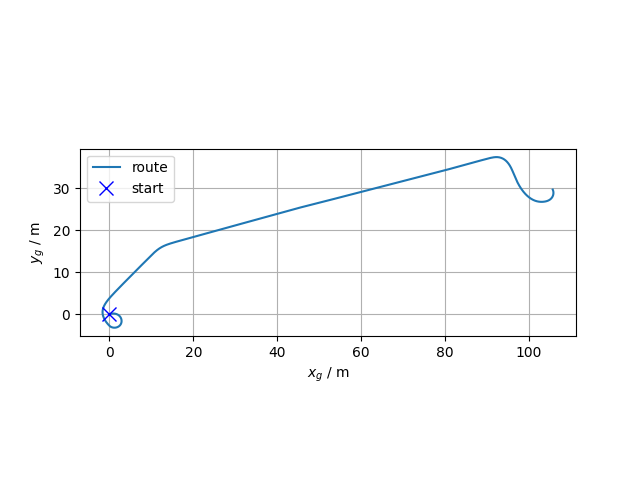
\includegraphics[width=\textwidth,trim={0.5cm 2cm 1.5cm 2.5cm },clip]{Figures/no-obstacle-no-waves-wind-5-10/position.png}
         \caption{No obstacle}
         \label{fig:no_obstacle_no_waves}
     \end{subfigure}
     \begin{subfigure}[b]{0.49\textwidth}
         \centering
         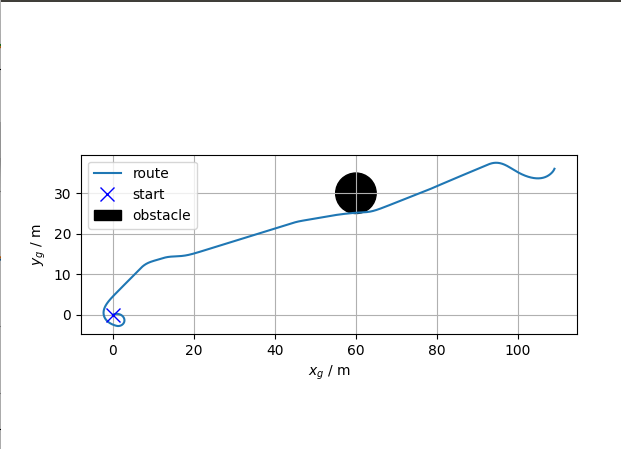
\includegraphics[width=\textwidth,trim={0.5cm 1cm 0.75cm 2.5cm },clip]{Figures/Obstacles-waves-wind-4-45/obsta.png}
         \caption{One obstacle}
         \label{fig:obstacle_no_waves}
     \end{subfigure}
    
     \hfill\\
     
    \caption{Sailing to \((x,y)=(100,40)\) with the wind in direction of sailing. No waves.}
    \label{fig:sail_with_wind}
\end{figure}
    
\end{frame}


\begin{frame}{Experiment: Obstacles with waves}
    \begin{figure}
     \centering
      \begin{subfigure}[b]{0.49\textwidth}
         \centering
         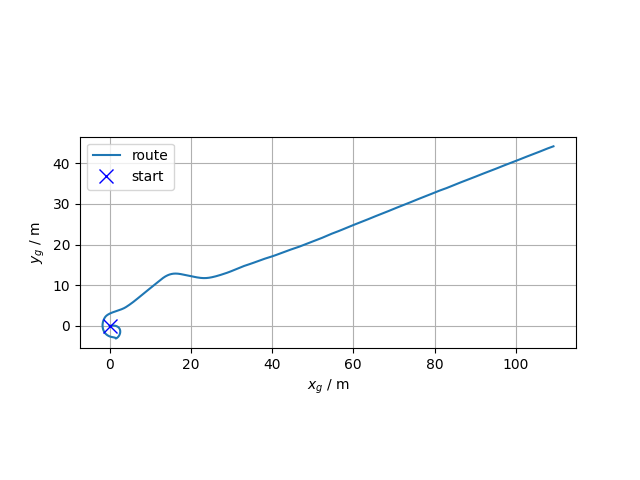
\includegraphics[width=\textwidth,trim={0.5cm 2cm 1.25cm 2.5cm },clip]{Figures/no-obstacle-waves-wind-5-65/position.png}
         \caption{No obstacles}
         \label{fig:no_obstacle_waves}
     \end{subfigure}
     \begin{subfigure}[b]{0.49\textwidth}
         \centering
         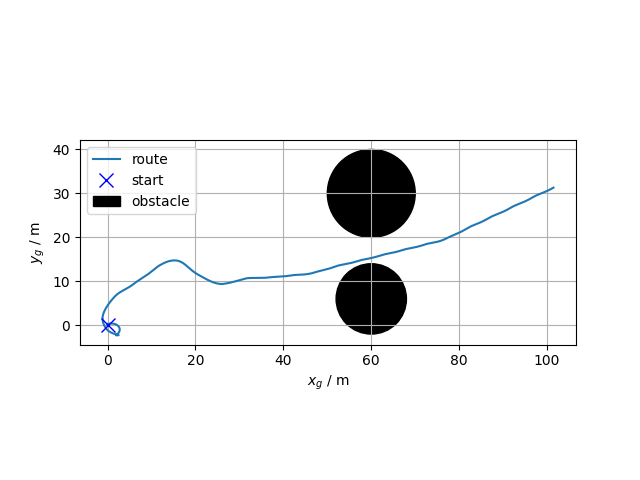
\includegraphics[width=\textwidth,trim={0.5cm 2cm 1.25cm 2.5cm },clip]{Figures/Obstacles-waves-wind-4-45/position-(with-waves).png}
         \caption{Two obstacles}
         \label{fig:obstacles_waves}
     \end{subfigure}
    
    \caption{Sailing to \((x,y)=(100,40)\) with the wind in direction of sailing. 0.5m Waves included.}
    \label{fig:sail_with_wind}
\end{figure}
\end{frame}
\begin{frame}{Experiment: Sailing with Wind}
    \begin{figure}
     \centering
     \begin{subfigure}[b]{0.4\textwidth}
         \centering
         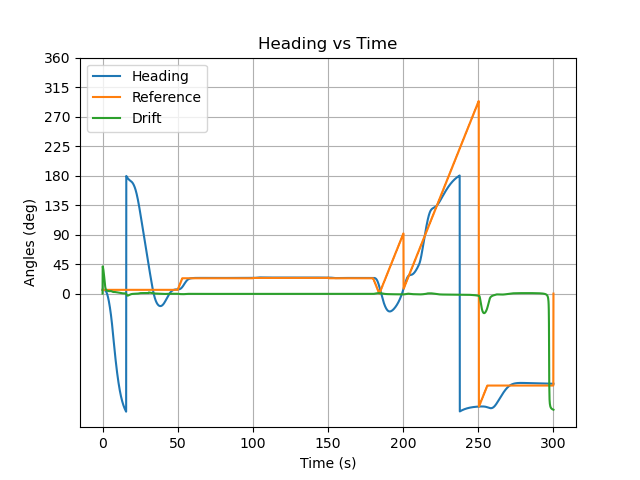
\includegraphics[width=\textwidth,trim={0.5cm 0.25cm 1.25cm 0.75cm },clip]{documents/final_pres_figs/with_wind_to_40_40_heading.png}
         \label{fig:with_wind_heading}
     \end{subfigure}
     \begin{subfigure}[b]{0.4\textwidth}
         \centering
         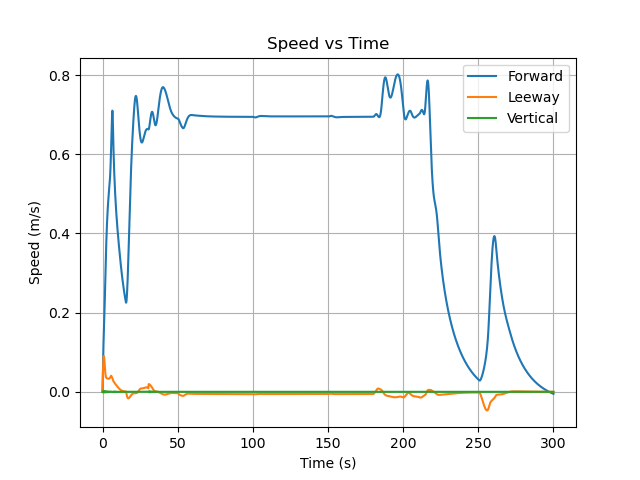
\includegraphics[width=\textwidth,trim={0.5cm 0.25cm 1.25cm 0.75cm },clip]{documents/final_pres_figs/with_wind_to_40_40_speed.png}
         \label{fig:with_wind_speed}
     \end{subfigure}
     \hfill\\
     \begin{subfigure}[b]{0.4\textwidth}
         \centering
         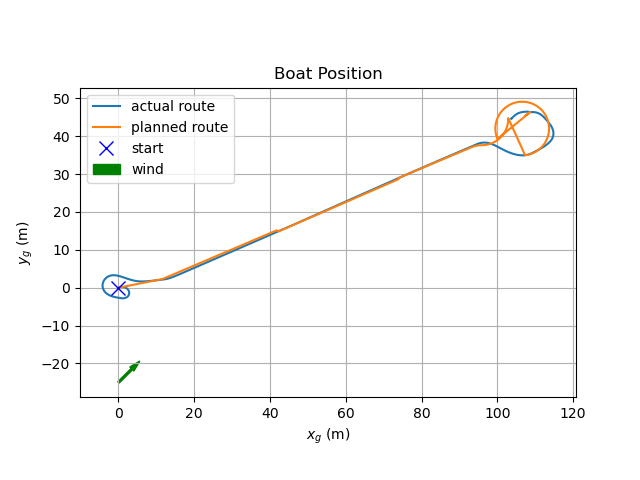
\includegraphics[width=\textwidth,trim={0.5cm 1cm 1.25cm 1.5cm },clip]{documents/final_pres_figs/with_wind_to_40_40_pos.png}
         \label{fig:with_wind_pos}
     \end{subfigure}
    \caption{Sailing to \((x,y)=(100,40)\) with the wind in direction of sailing. No waves.}
    \label{fig:sail_with_wind}
\end{figure}
\end{frame}

\begin{frame}{Experiment: Sailing with Crosswinds}
    \begin{figure}
     \centering
     \begin{subfigure}[b]{0.35\textwidth}
         \centering
         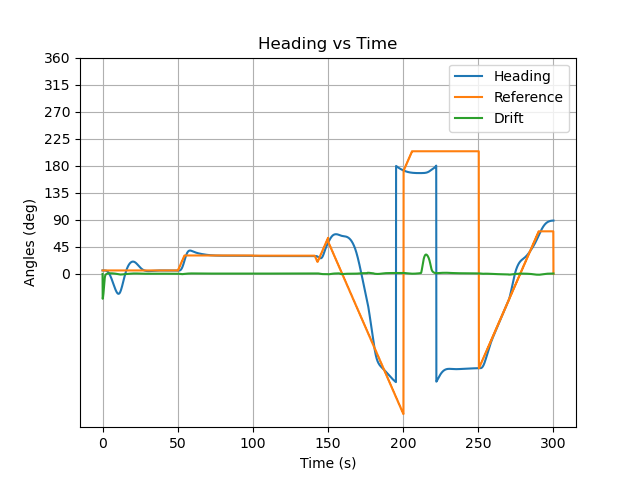
\includegraphics[width=\textwidth,trim={0.5cm 0.25cm 1.25cm 0.75cm },clip]{documents/final_pres_figs/right_to_wind_to_40_40_heading.png}
         \label{fig:right_wind_heading}
     \end{subfigure}
     \begin{subfigure}[b]{0.35\textwidth}
         \centering
         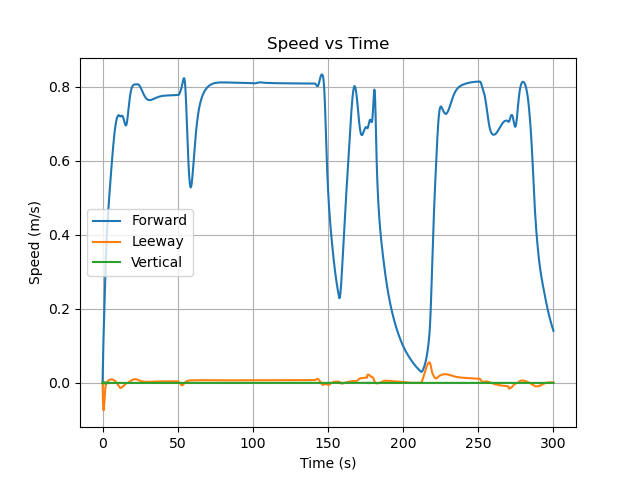
\includegraphics[width=\textwidth,trim={0.5cm 0.25cm 1.25cm 0.75cm },clip]{documents/final_pres_figs/right_to_wind_to_40_40_speed.png}
         \label{fig:right_wind_speed}
     \end{subfigure}
     \hfill\\
     \begin{subfigure}[b]{0.4\textwidth}
         \centering
         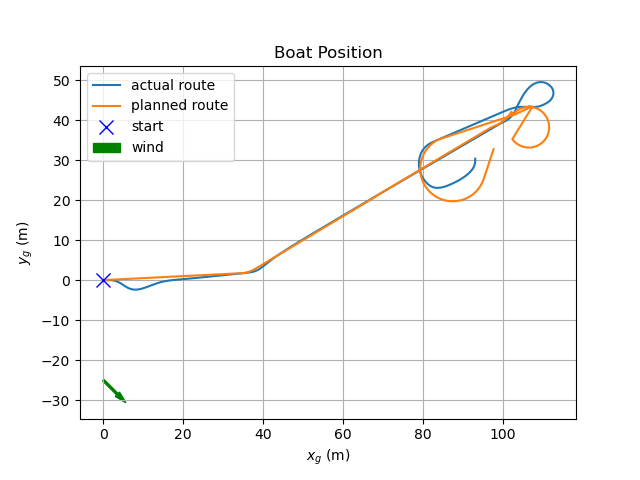
\includegraphics[width=\textwidth,trim={0.5cm 0.25cm 1.25cm 0.75cm },clip]{documents/final_pres_figs/right_to_wind_to_40_40_pos.png}
         \label{fig:right_wind_pos}
     \end{subfigure}
    \caption{Sailing to \((x,y)=(100,40)\) with the winds cross to direction of sailing. No waves.}
    \label{fig:sail_crosswind}
\end{figure}
\end{frame}

\begin{frame}{Experiment: Sailing Against Wind}
    \begin{figure}
     \centering
     \begin{subfigure}[b]{0.33\textwidth}
         \centering
         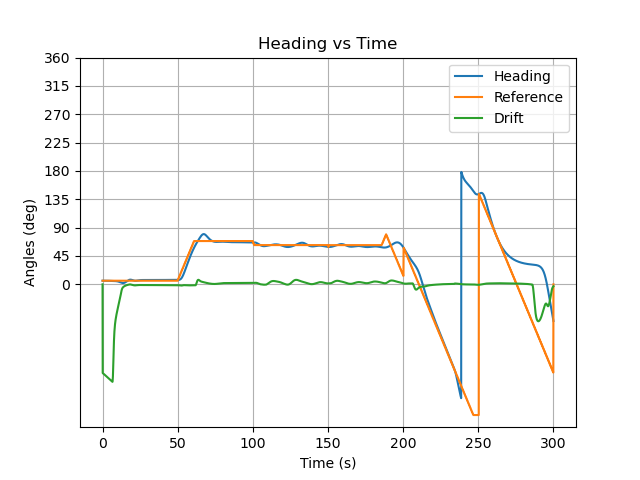
\includegraphics[width=\textwidth,trim={0.5cm 0.25cm 1.25cm 0.75cm },clip]{documents/final_pres_figs/against_wind_to_40_40_heading.png}
         \label{fig:right_wind_heading}
     \end{subfigure}
     \begin{subfigure}[b]{0.33\textwidth}
         \centering
         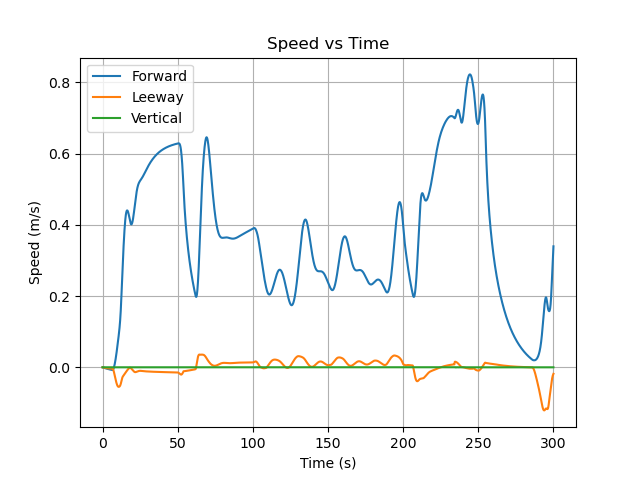
\includegraphics[width=\textwidth,trim={0.5cm 0.25cm 1.25cm 0.75cm },clip]{documents/final_pres_figs/against_wind_to_40_40_speed.png}
         \label{fig:right_wind_speed}
     \end{subfigure}
     \hfill\\
     \begin{subfigure}[b]{0.4\textwidth}
         \centering
         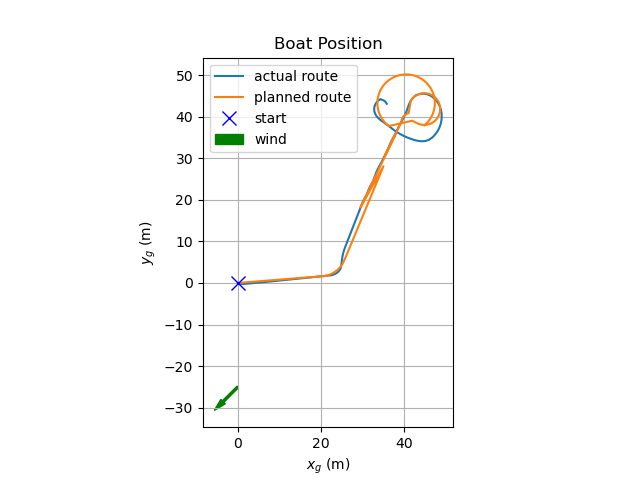
\includegraphics[width=\textwidth,trim={0.5cm 0.0cm 1.25cm 0.5cm },clip]{documents/final_pres_figs/against_wind_to_40_40_pos.png}
         \label{fig:right_wind_pos}
     \end{subfigure}
    \caption{Sailing to \((x,y)=(40,40)\) with the winds against direction of sailing. No waves.}
    \label{fig:sail_against_wind}
\end{figure}
\end{frame}

% \begin{frame}{Experiment: Planning with Obstacles}
%     without waves.
    
%     at least show position plan with versus without obstacle.
% \end{frame}

% \begin{frame}{Experiment: Planning with Obstacles}
%     with waves
    
%     show position plan with versus without obstacles, and also show effect of waves with some plot
% \end{frame}




\section{Conclusion}

\begin{frame}{Future Work and Improvements}

\begin{itemize}
    \item Improve simplified planner boat dynamics model:
    \begin{itemize}
        \item Speed up planner.
        \item More accurately model boat velocity.
        \item More accurately model or predict environment (to better handle environmental disturbances).
    \end{itemize}
    \item Expand obstacle model to support:
        \begin{itemize}
            \item More complex geometries.
            \item Simple dynamics like drifting in water.
        \end{itemize}
\end{itemize}
    
\end{frame}

\begin{frame}{Conclusion}
    In our project we develop and present an optimization-based planner for generating
    reference headings from high-level position targets, to pass to yaw controllers, which are more developed in literature.
    
    \hfill\\
    The optimization-based planner is flexible enough to handle additional constraints such as  obstacle avoidance, and is fast enough to allow for replanning to create a closed-loop planning and control system.
    
    \hfill\\
    Modular design where planner and yaw controller blocks can be switched out.
    
    \hfill\\
    Sailboat simulator library which is modular and usable for testing planners and controllers.
\end{frame}

\begin{frame}{Thank You}
    Questions?
\end{frame}


\begin{frame}{References}
    \printbibliography{}
\end{frame}

\end{document}